\documentclass{beamer}
\usepackage[magyar]{babel}
\usepackage[utf8]{inputenc}
\usepackage[T1]{fontenc}
\usepackage{graphicx, tikz, multicol, wrapfig}
\usepackage[framemethod=TikZ]{mdframed}


\mode<presentation>
{
    \usetheme{Boadilla}
    \usecolortheme{default}
    \usefonttheme{default}
    \setbeamertemplate{navigation symbols}{}
    \setbeamertemplate{caption}[numbered]
}

\newcommand\figu[3]{
    \begin{figure}
        \includegraphics[width=#2\textwidth]{#1}
        \caption{#3}
    \end{figure}
}


\title[Komplex viszga, ELTE]{Műholdradar interferometria és GNSS mérések
                             kombinálása 3D-s deformációs terek meghatározására}
\author[Bozsó István]{Bozsó István}
\institute[MTA CSFK GGI]{MTA CSFK Geodéziai és Geofizikai Intézet; ELTE Földtudományi Doktori Iskola}
\date{2019.05.30.}

\def\rar{\rightarrow}
\def\lar{\leftarrow}

\newcommand\quo[1]{``#1''}
\newcommand\subt[2]{#1_{\text{#2}}}
\newcommand\pard[2]{\frac{\partial #1}{\partial #2}}
\newcommand\abs[1]{\left|#1\right|}


\newcommand\inc[1] {
    \includegraphics[width=\textwidth]{#1}
}

\newcommand\img[2] {
    \includegraphics[width=#2\textwidth]{#1}
}

\newenvironment{ffig}[1]
{
    \begin{mdframed}[linecolor=#1, linewidth=5.0pt, roundcorner=5pt,
                     innerrightmargin=10pt, innerleftmargin=10pt,
                     innertopmargin=0pt, innerbottommargin=5pt,
                     skipabove=0pt, skipbelow=0pt,
                     backgroundcolor=white, frametitle={}, align=center]
    \begin{center}
}
{
    \end{center}
    \end{mdframed}
}

\newenvironment{fig}[1]
{
    \begin{minipage}{#1\textwidth}
    \begin{center}
}
{
    \end{center}
    \end{minipage}
}


\newcommand{\fcap}[1] {
    \captionof{figure}{#1}
}

\newcommand{\genenv}[1] {
    \def\b#1 { \begin{#1} }
    \def\e#1 { \end{#1} }
}


\def\bffig { \begin{ffig} }
\def\effig {   \end{ffig} }

\def\bfig { \begin{fig} }
\def\efig {   \end{fig} }

\def\bitz { \begin{itemize} }
\def\eitz {   \end{itemize} }

\def\bmini { \begin{minipage} }
\def\emini {   \end{minipage} }

\def\bcent { \begin{center} }
\def\ecent {   \end{center} }

\def\fcol{\color{blue!55!black}}

\newcommand{\fig}[1]{
    \begin{mdframed}[linecolor=blue!65!white, linewidth=1.75pt, roundcorner=0.75pt,
                     innerrightmargin=0pt, innerleftmargin=0pt,
                     innertopmargin=0pt, innerbottommargin=0pt,
                     backgroundcolor=white, frametitle={}, align=center]
        \includegraphics[width=1.0\textwidth]{#1}
    \end{mdframed}
}

\newcommand{\figm}[2]{
    \begin{center}
    \begin{minipage}[c]{#2\textwidth}
    \begin{mdframed}[linecolor=blue!65!white, linewidth=1.75pt, roundcorner=0.75pt,
                     innerrightmargin=0pt, innerleftmargin=0pt,
                     innertopmargin=0pt, innerbottommargin=0pt,
                     backgroundcolor=white, frametitle={}, align=center]
        \includegraphics[width=1.0\textwidth]{#1}
    \end{mdframed}
    \end{minipage}
    \end{center}
}

\newenvironment{minic}[1]
{
    \begin{center}
    \begin{minipage}[c]{#1\textwidth}
}
{
    \end{minipage}
    \end{center}
}


\newenvironment{figp}[4]
{
    \begin{minipage}[c]{#3\textwidth}
    \centering
    #1
    
    #2
    \end{minipage}
    \begin{minipage}[c]{#4\textwidth}
}
{
    \end{minipage}
}


\newcommand{\figc}[2]
{
    \begin{center}
    \begin{mdframed}[linecolor=blue!65!white, linewidth=1.75pt, roundcorner=0.75pt,
                     innerrightmargin=0pt, innerleftmargin=0pt,
                     innertopmargin=0pt, innerbottommargin=0pt,
                     backgroundcolor=white, frametitle={}, align=center]
    
    \includegraphics[width=1.0\textwidth]{#1}
    \end{mdframed}
    #2
    \end{center}
}

\newcommand\sepframe[1] {
    \begin{frame}
        \begin{center}
            \Huge \fcol
            #1
        \end{center}
    \end{frame}
}


\graphicspath{{../images/}}


\begin{document}

\begin{frame}
    \titlepage
    \begin{center}
        \begin{minipage}[c]{0.3\textwidth}
            
\includegraphics[width=0.75\textwidth]{ggi_logo.png}
        \end{minipage}
        \begin{minipage}[c]{0.3\textwidth}
            
\includegraphics[width=0.75\textwidth]{elte_logo.png}
        \end{minipage}
    \end{center}
\end{frame}


\begin{frame}{Szintetikus Apertúrájú Radarinterferometria - InSAR}

\begin{itemize}
    \item szintetikus apertúrájú radar - mikrohullám tartományban működő
    távérzékelési rendszer (műhold, repülő, drone)
    \item felszíni deformációk nagyfelbontású térképezése
    \item fedetlen felszínen potenciálisan több 1000, több 100 000 reflektáló pont
    \item relatív módszer, térben, időben
    \item felszíni deformáció mérés hibája ideális esetben $< \text{mm}$,
    gyakorlatban általában elmondható $< \text{cm}$
    \item tektonikus, eróziós folyamatok; emberi tevékenység okozta
    deformációk térképezése, monitorozása
    \item kritikus infrastruktúra megfigyelése (gátak, veszélyes hulladék
    tározók)
    \item geodinamikai szempontból felbecsükhetetlen jelentőség, komplex
    dinamikai mintázattal rendelkező területek hosszútávú megfigyelése
    \item ESA műholdas földmegfigyelési programjában kiemelt szerep
    (Sentinel-1 A/B)
\end{itemize}

\end{frame}


\begin{frame}{InSAR alapelv}
    %\begin{minipage}[c]{0.475\textwidth}
    %    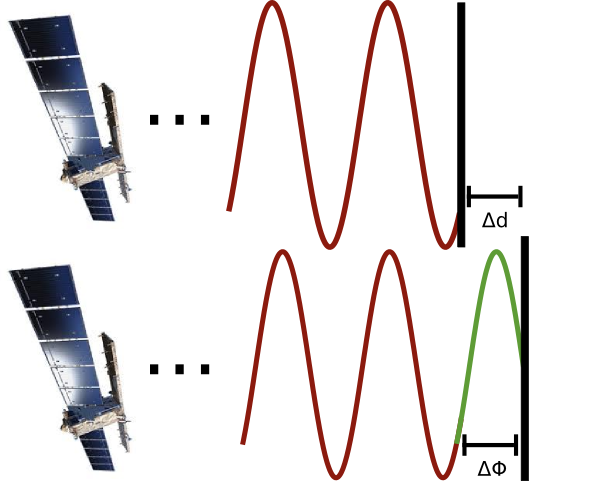
\includegraphics[width=\textwidth]{interfero.png}
    %\end{minipage}
    %\begin{minipage}[c]{0.475\textwidth}
    %    \begin{itemize}
    %        \item $\Delta d = \frac{\lambda}{4\pi} \Delta \Phi$
    %        \item 
    %    \end{itemize}
    %\end{minipage}
    
    \begin{center}
        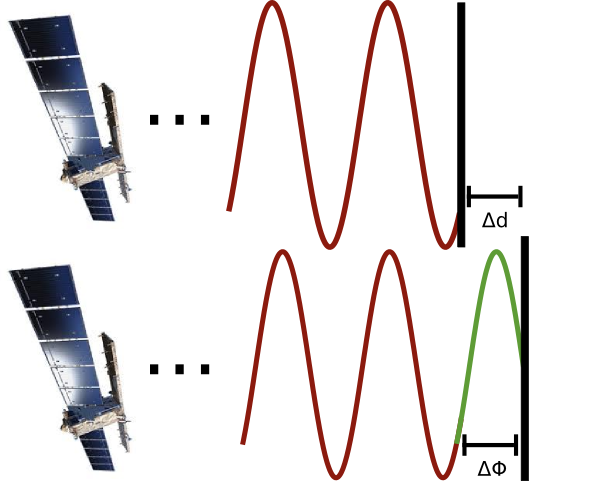
\includegraphics[width=0.7\textwidth]{interfero.png}
        
        $\Delta d = \frac{\lambda}{4\pi} \Delta \Phi$
    \end{center}
\end{frame}

\begin{frame}{Példa interferogramok}

    \begin{center}
        \figu{hun_nkp1.png}{0.9}{Koherens, téli, interferogramok}
    \end{center}

\end{frame}

\begin{frame}{Példa interferogramok}

    \begin{center}
        \figu{hun_nkp3.png}{0.9}{Inkoherens, nyári, interferogramok}
    \end{center}

\end{frame}

\begin{frame}{InSAR korlátai}

\begin{table}
\begin{tabular}{| c | c | c |} \hline
Sáv elnevezése & Frekvencia $[\text{GHz}]$ & Hullámhossz $[\text{cm}]$ \\ \hline \hline
X & 8.0 -- 12.0 & 3.75 -- 2.5 \\ \hline
C & 4.0 -- 8.0 & 7.5 -- 3.75 \\ \hline
L & 1.0 -- 2.0 & 30 -- 15 \\ \hline
\end{tabular}
\end{table}

\begin{itemize}
    \item felszíni elmozdulás műholdirányú vetülete mérhető csak
    (felszálló - ascending, leszálló - descending műholdáthaladás)
    \item felszín reflexiós tulajdonságai időben változnak - jel koherenciája
    elvész (pl. vegetációval sűrűn fedett terület - X,C sáv, hó, homok, talaj
    nedvességtartalma)
    \item visszatérési idő: 6-12 vagy több nap
    \item egyéb hullámterjedést befolyásoló tényezők szűrése: semleges
    atmoszférában, ionoszférában az EM hullám terjedési sebességének változása
    \item cél: fenti limitációkat hatását kiküszöbölni - reflektor, atmoszféra
    és ionoszféra modellek, szűrési módszerek
\end{itemize}

\end{frame}


\begin{frame}{GGI - Űrgeodézia Kutatócsoport}

\begin{itemize}
    \item InSAR alkalmazási területeinek kiterjesztése
    \item mesterséges reflektáló pontok kifejlesztése
    (geometria optimalizálása), sarokreflektor
    \item InSAR elmozdulások kombinálása GPS mérésekkel $\rightarrow$ 3D elmozdulás
    \item jelterjedés vizsgálata, atmoszférikus, ionoszférikus hatások
    \item GGI: ionoszonda - kísérleti üzem, kísérleti eredmények; hozzáférés
    globális ionoszonda hálózathoz
    \item InSAR regionális alkalamzások - első eredmények (Kelet-Magyarország)
\end{itemize}

\end{frame}


\begin{frame}{GGI - Űrgeodézia Kutatócsoport}

\begin{itemize}
    \item reflektorhálózatok, területek, ahol nincs vagy csak kevés
    koherens szórópont
    \item Magyarországon: 3 + 1 sarokreflektor hálózat (Fonyód, Kulcs, Dunaszekcső, Sopron)
    \item Erdélyben: 2 sarokreflektor hálózat (Parajd, Csomád);
    1 tervezett (Vrancea-zóna)
    \item eltérő felszínmozgási folyamatok (földcsuszamlás, sótektonika,
    posztvulkáni tevékenység, szubdukció)
    \item ESA-PECS projekt keretérben kifejlesztett ISIGN programrendszer
    InSAR és GPS adatok kombinálására
\end{itemize}

\end{frame}


\begin{frame}{Sarokreflektorok}

\begin{center}
    \figu{dszekcso_refl_3.jpg}{0.75}{Dunaszekcsői reflektorhálózat egyik
          ikerreflektora, GNSS adapterrel}
\end{center}

\begin{itemize}
    \item több reflektor $\rightarrow$ reflektor hálózat
    \item elmozdulások egy kijelölt stabil referencia reflektorhoz képest
    \item mm alatti pontosság elérhető
\end{itemize}

\end{frame}


\begin{frame}{Erdélyi hálózatok}
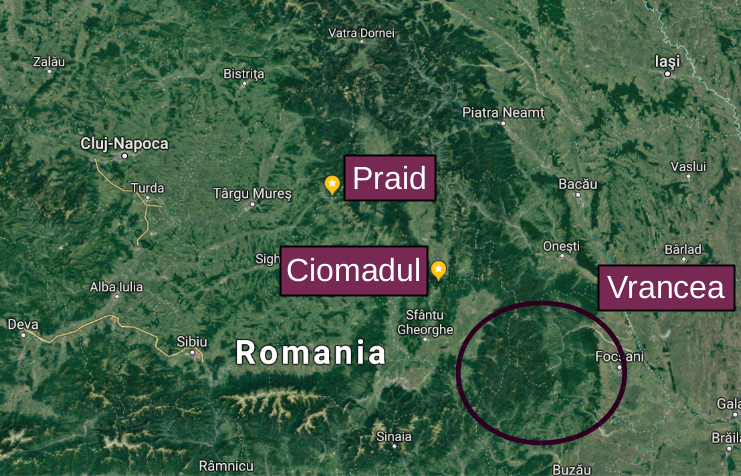
\includegraphics[width=0.9\textwidth]{praid_ciomadul.png}
\end{frame}


\begin{frame}{Parajdi hálózat}
    \begin{minipage}[c]{0.475\textwidth}
        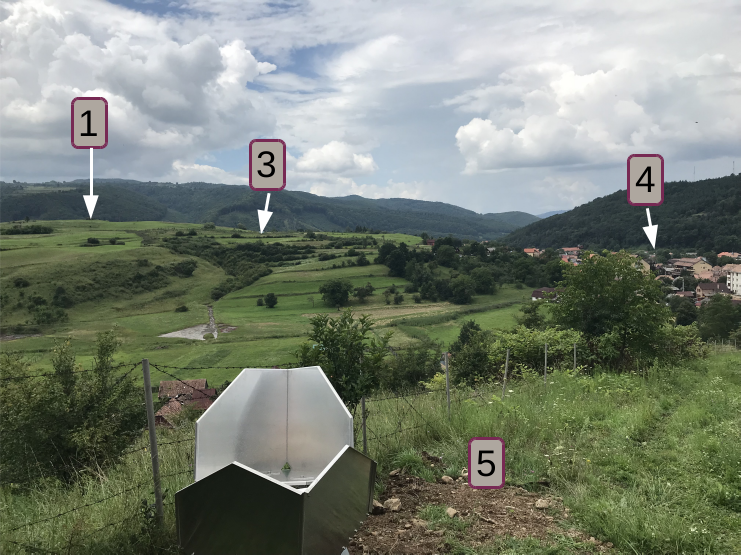
\includegraphics[width=\textwidth]{praid_refl.png}
    \end{minipage}
    \begin{minipage}[c]{0.475\textwidth}
        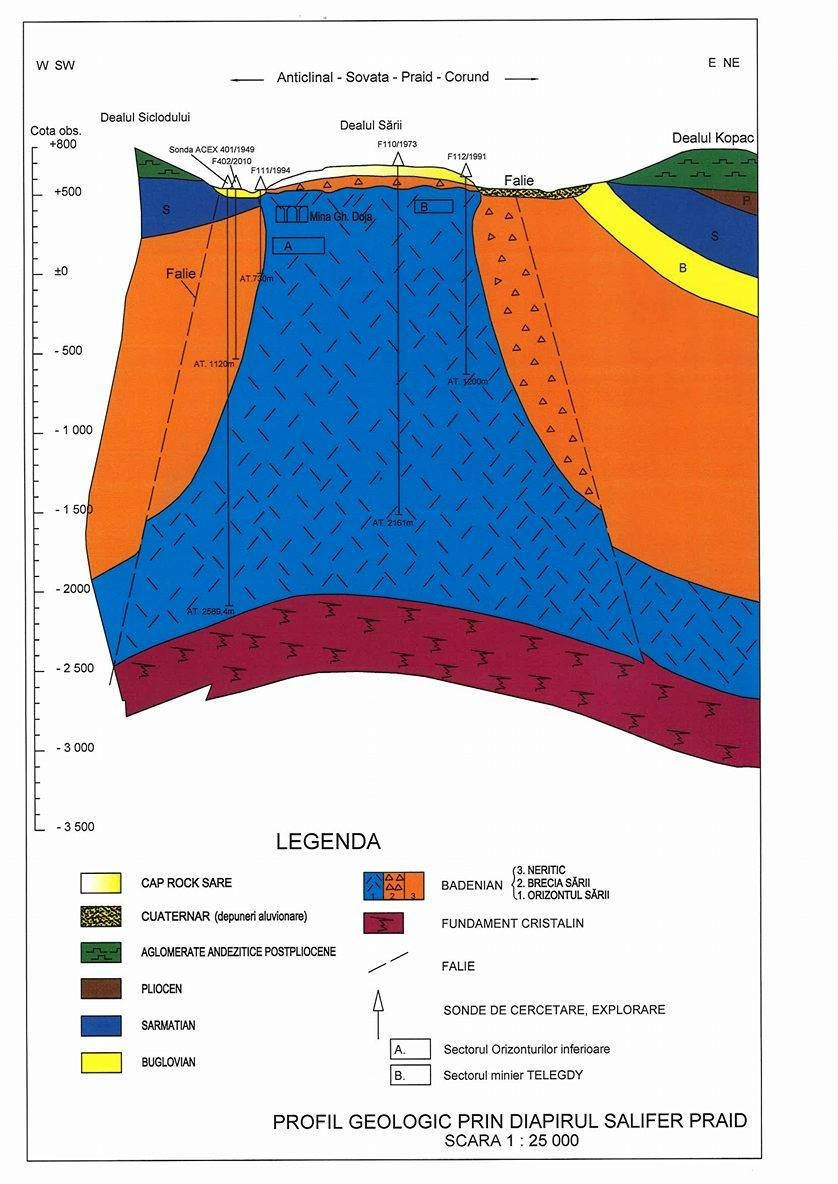
\includegraphics[width=\textwidth]{praid_schematic.png}
    \end{minipage}
\end{frame}


\begin{frame}{Parajdi hálózat}
\figu{parajd_ts1.png}{0.9}{Sósziklák deformációs idősora}
\end{frame}

\begin{frame}{Parajdi hálózat}
\figu{parajd_ts2.png}{0.9}{1-es reflektor deformációs idősora}
\end{frame}

\begin{frame}{Parajdi hálózat}
\figu{parajd_ts3.png}{0.9}{2-es reflektor deformációs idősora}
\end{frame}

\begin{frame}{Parajdi hálózat}
\figu{parajd_ts4.png}{0.9}{3-as reflektor deformációs idősora}
\end{frame}


\begin{frame}{Magyarországi hálózatok}
    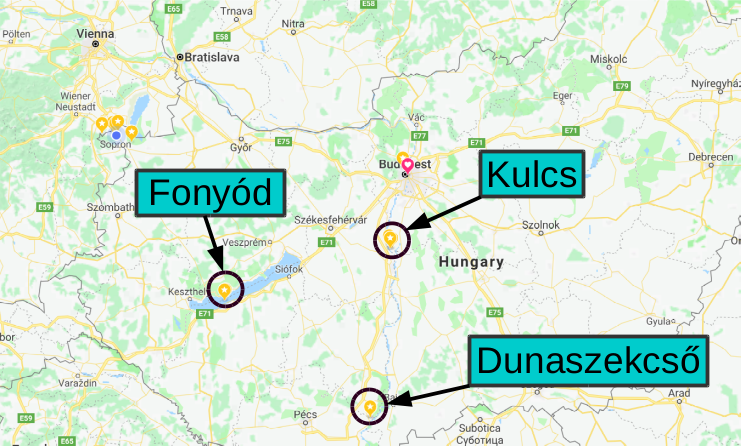
\includegraphics[width=0.9\textwidth]{hungary_networks.png}
\end{frame}

\begin{frame}{Magyarországi hálózatok}

\begin{minipage}[c]{0.975\textwidth}
    \begin{minipage}[c]{0.47\textwidth}
        \figu{IB2-IB1_kalman.pdf}{1.0}{Dunszakcső, IB2 - IB1}
    \end{minipage}
    \begin{minipage}[c]{0.47\textwidth}
        \figu{A1-AR_kalman.pdf}{1.0}{Kulcs, A1 - AR}
        %\includegraphics[width=\textwidth]{}
    \end{minipage}
\end{minipage}
\begin{minipage}[c]{0.975\textwidth}
    \begin{minipage}[c]{0.47\textwidth}
        \figu{KV-PH_kalman.pdf}{1.0}{Fonyód, VK - PH}
        %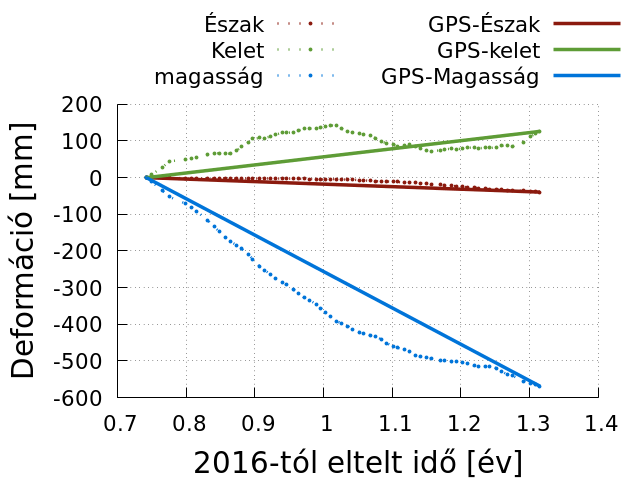
\includegraphics[width=\textwidth]{IB4-IB1_kalman.png}
    \end{minipage}
    \begin{minipage}[c]{0.475\textwidth}
        \begin{itemize}
            \item különböző dinamika
            \item korreláció meteorológiával?
            \item epizodikus vislkedés
        \end{itemize}
    \end{minipage}
\end{minipage}
\end{frame}


\begin{frame}{Kelet-Magyarországi regionális vizsgálat első eredményei}
    \begin{minipage}[c]{0.675\textwidth}
        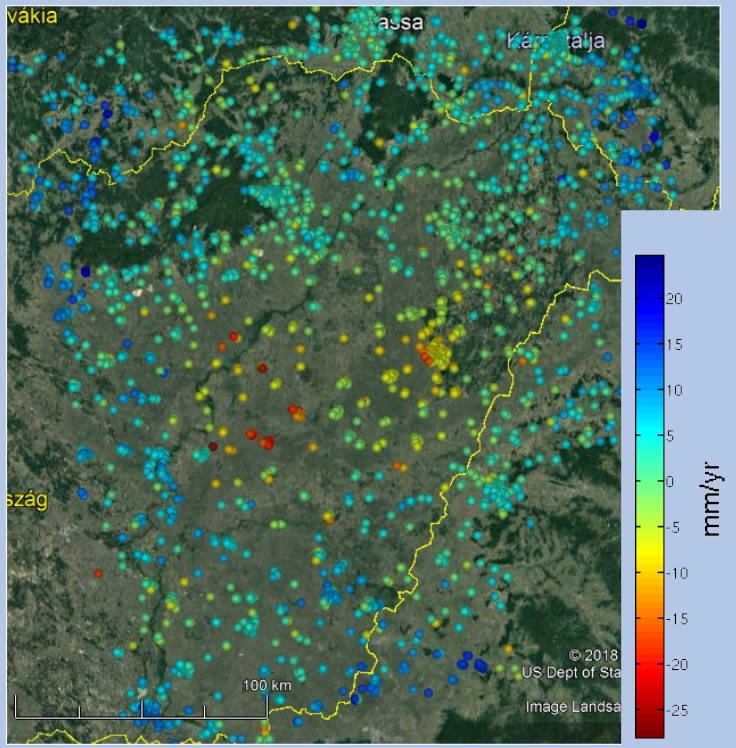
\includegraphics[width=1.0\textwidth]{hun_nkp2.png}
    \end{minipage}
    \hspace{10pt}
    \begin{minipage}[c]{0.25\textwidth}
        3.5 éves Sentinel-1 adatsor, előzetes eredmények
    \end{minipage}
\end{frame}


\begin{frame}{Kutatási- és publikációs terv}

\begin{itemize}
    \item ISIGN programrendszer továbbfejlesztése, atmoszférikus
    és ionoszférikus korrekciók beépítése
    \item további reflektorhálózatok telepítése, meglévő hálózatok adatainak
    feldolgozása, eredmények értelmezése
    \item reflektorhálózatok feldolgozási eredményeinek publikálása
    \item nem mozgó területeken atmoszféra, ionoszféra vizsgálata
\end{itemize}

\end{frame}


\begin{frame}{Publikációk}
    \bibliography{/home/istvan/Dokumentumok/texfiles/insar}
    \bibliographystyle{apalike}
\end{frame}

\begin{frame}
    \begin{center}
        \Huge \fcol
        Köszönöm a figyelmet!
    \end{center}
    \vspace{25pt}
    
    \begin{center}
        \Large \center Köszönettel tartozom:
        
        Szűcs Eszter, Lichtenberger János, Wesztergom Viktor, Bányai László
    \end{center}
    \vspace{10pt}

\end{frame}



\begin{frame}{Integrált Vízgőzmennyiség}
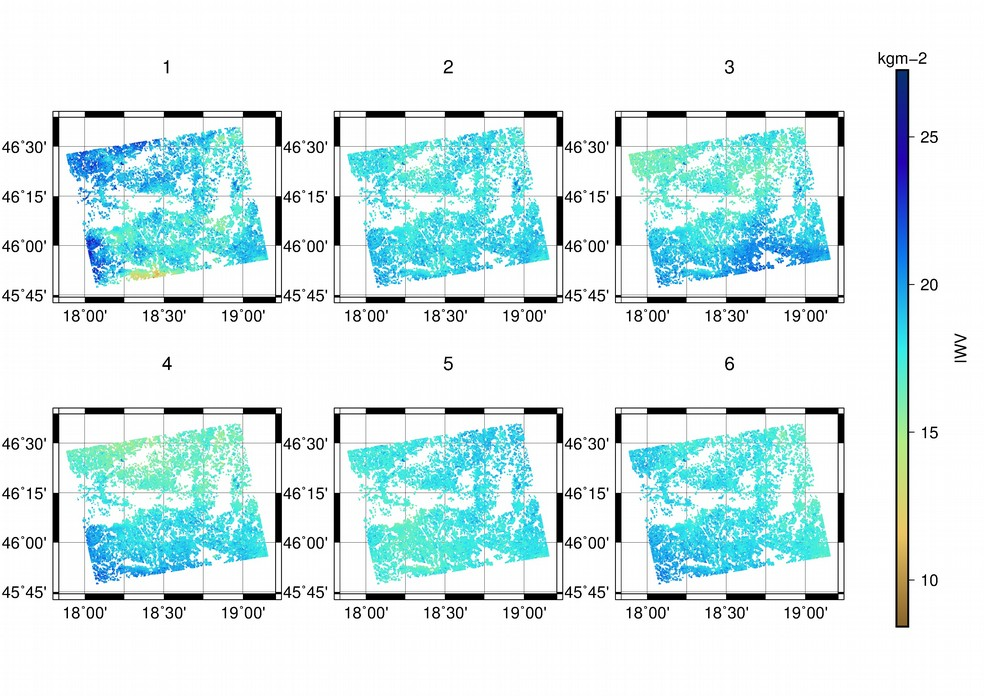
\includegraphics[width=0.9\textwidth]{iwv.png}
\end{frame}


\begin{frame}{Integrált Elektrontartalom változás}
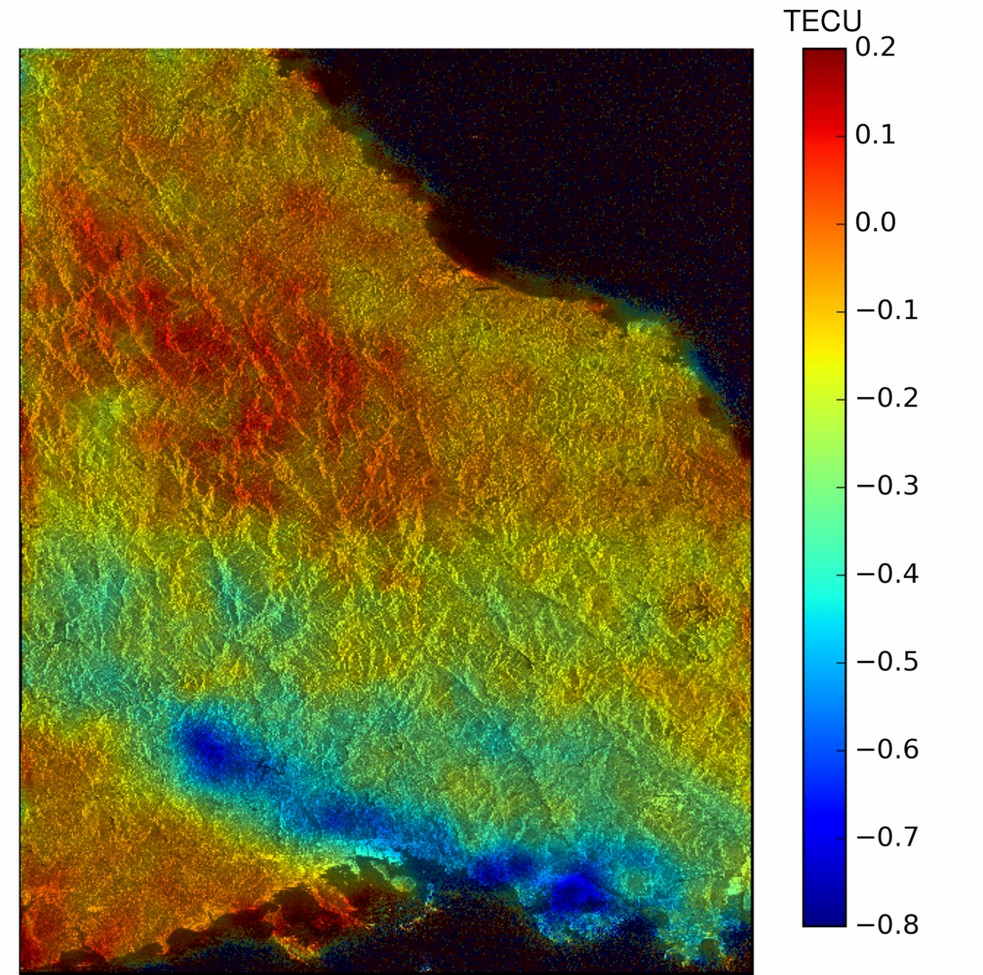
\includegraphics[width=0.7\textwidth]{iono.png}
\end{frame}

\begin{frame}{}
\cite{Szucs2018, banyai2018mHuholdradar}
\end{frame}


\end{document}